\documentclass{article}
\usepackage[x11names, rgb]{xcolor}
\usepackage[utf8]{inputenc}
\usepackage{tikz}
\usetikzlibrary{snakes,arrows,shapes}
\usepackage{amsmath}
%
%

%

%

\begin{document}
\pagestyle{empty}
%
%
%

\enlargethispage{100cm}
% Start of code
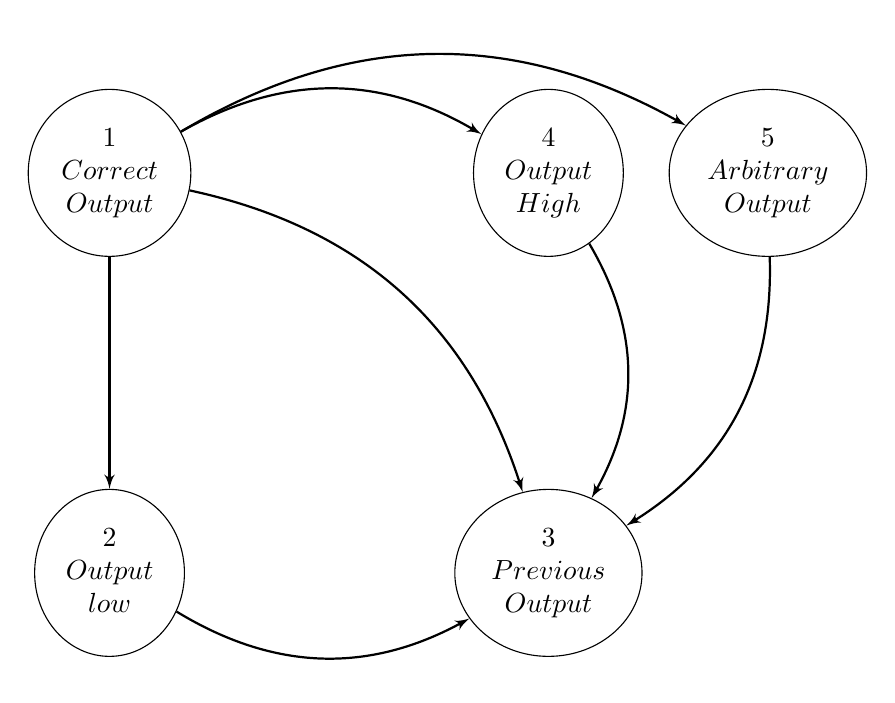
\begin{tikzpicture}[>=latex',line join=bevel,]
%%
\node (1) at (27bp,162bp) [draw,ellipse] {$\begin{matrix}1 \\ Correct \\ Output\end{matrix}$};
  \node (3) at (185bp,18bp) [draw,ellipse] {$\begin{matrix}3 \\ Previous \\ Output\end{matrix}$};
  \node (2) at (27bp,18bp) [draw,ellipse] {$\begin{matrix}2 \\ Output \\ low\end{matrix}$};
  \node (5) at (264bp,162bp) [draw,ellipse] {$\begin{matrix}5 \\ Arbitrary \\ Output\end{matrix}$};
  \node (4) at (185bp,162bp) [draw,ellipse] {$\begin{matrix}4 \\ Output \\ High\end{matrix}$};
  \coordinate (7) at (106bp,18bp);
  \coordinate (8) at (106bp,162bp);
  \draw [->,thick] (2) to[bend right] (3);
  \draw [->,thick] (1) to[bend left] (4);
  \draw [->,thick] (5) to[bend left] (3);
  \draw [->,thick] (1) to[bend left] (5);
  \draw [->,thick] (1) ..controls (27bp,119.2bp) and (27bp,75.247bp)  .. (2);
  \draw [->,thick] (4) to[bend left] (3);
  \draw [->,thick] (1) to[bend left] (3);
%
\end{tikzpicture}
% End of code

%
\end{document}
%



